\documentclass{article}
\usepackage{graphicx}
\usepackage[dvipsnames,table]{xcolor}
\usepackage[utf8]{inputenc}
\usepackage{siunitx}
\usepackage[american,siunitx]{circuitikz}
\usepackage{amsmath}
\usepackage{svg}
\usepackage{booktabs}
\usepackage{float}
\usepackage{xparse, xfp}
\usepackage{multirow}
\usepackage{tikz}
\usepackage{karnaugh-map}
\usepackage{pdfpages}
\usepackage{hyperref}
\hypersetup{
    colorlinks=true,
    linkcolor=blue,
    filecolor=magenta,      
    urlcolor=cyan,
}
\usetikzlibrary{calc}
%\usepackage[landscape]{geometry}
\renewcommand{\thesubsection}{\thesection.\alph{subsection}}
\newcommand{\equal}{=}
\newcommand{\greyrule}{\arrayrulecolor{black!30}\midrule\arrayrulecolor{black}}
\makeatletter
\newcommand\currcoor{\the\tikz@lastxsaved,\the\tikz@lastysaved}
\makeatother
\newcolumntype{:}{@{\hskip\tabcolsep\color{black!30}\vrule\hskip\tabcolsep}}

\ExplSyntaxOn
\NewExpandableDocumentCommand \groupify { O{\,\allowbreak} m m }
  { \jakob_groupify:nnn {#1} {#2} {#3} }
\cs_new:Npn \jakob_groupify:nnn #1 #2 #3
  { \__jakob_groupify_loop:nnw { 1 } {#2} #3 \q_recursion_tail {#1} \q_recursion_stop }
\cs_new:Npn \__jakob_groupify_loop:nnw #1 #2 #3
  {
    \quark_if_recursion_tail_stop:n {#3}
    \exp_not:n {#3}
    \int_compare:nNnTF {#1} = {#2}
      { \__jakob_groupify_sep:n }
      { \exp_args:Nf \__jakob_groupify_loop:nnw { \int_eval:n { #1+1 } } }
          {#2}
  }
\cs_new:Npn \__jakob_groupify_sep:n #1 #2 \q_recursion_tail #3
  {
    \tl_if_empty:nF {#2} { \exp_not:n {#3} }
    \__jakob_groupify_loop:nnw { 1 } {#1}
    #2 \q_recursion_tail {#3}
  }
\ExplSyntaxOff

\title{ECE 2200L\\Introduction to Microelectronics Circuits Laboratory\\\,\\Experiment 4\\Zener Diode I-V Characteristics\\\,\\Report}
\author{Choi Tim Antony Yung}
\begin{document}
\maketitle

\thispagestyle{empty}
\setcounter{page}{0}

\newpage

\section*{Objective}

To study the current-voltage relationship of a Zener diode, to determine the reverse saturation current, the ideality factor ($\eta$) in the forward region, the Zener voltage and the Zener resistance ($R_Z$) in the Zener region.

\section*{Result}
The following is the experimental data obtained from 1N4733 Zener diode.
\begin{table}[H]
  \centering
    \begin{tabular}{rrrrr}
    \toprule
    &\multicolumn{1}{c}{$V_d$ (V)} & \multicolumn{1}{c}{$I_d$ (A)} & \multicolumn{1}{c}{$\frac{V_d}{V_T}$} & \multicolumn{1}{c}{$ln(I_d)$ (A)} \\
    \midrule
    \multirow{4}[0]{*}{Reverse Breakdown} & -5.175 & -3.051$\times10^{-2}$ & \multicolumn{2}{c}{\multirow{4}[0]{*}{N/A}} \\
          & -5.137 & -1.808$\times10^{-2}$ & \multicolumn{2}{c}{} \\
          & -5.112 & -1.034$\times10^{-2}$ & \multicolumn{2}{c}{} \\
          & -5.089 & -4.790$\times10^{-3}$ & \multicolumn{2}{c}{} \\
          \midrule
    \multirow{6}[0]{*}{Reverse Bias} & -4.749 & -2.200$\times10^{-4}$ & \multicolumn{2}{c}{\multirow{6}[0]{*}{N/A}} \\
          & -4.553 & -1.031$\times10^{-4}$ & \multicolumn{2}{c}{} \\
          & -3.568 & -5.500$\times10^{-6}$ & \multicolumn{2}{c}{} \\
          & -2.088 & -2.000$\times10^{-7}$ & \multicolumn{2}{c}{} \\
          & -1.055 & -1.000$\times10^{-7}$ & \multicolumn{2}{c}{} \\
          & 0.337  &  0.000$\times10^{+0}$ & \multicolumn{2}{c}{} \\
    \midrule
    \multirow{7}[0]{*}{Forward Bias} & 0.654 & 1.570$\times10^{-4}$ & 25.15385 & -8.75926 \\
          & 0.753 & 4.355$\times10^{-3}$ & 28.96154 & -5.43643 \\
          & 0.772 & 8.420$\times10^{-3}$ & 29.69231 & -4.77715 \\
          & 0.783 & 1.218$\times10^{-2}$ & 30.11538 & -4.40796 \\
          & 0.793 & 1.657$\times10^{-2}$ & 30.50000 & -4.10016 \\
          & 0.799 & 2.067$\times10^{-2}$ & 30.73077 & -3.87907 \\
          & 0.805 & 2.494$\times10^{-2}$ & 30.96154 & -3.69128 \\
    \bottomrule
  \end{tabular}
\end{table}

From the $\frac{V_d}{V_T}$ vs $ln(I_d)$ chart (\ref{fig:log}), the ideality of the diode $\eta$ can be derived from reciprocal of the slope of line of best fit: $$\eta=\frac{1}{0.8739}=1.144$$
% and the saturation current $I_s$ can be derived by taking the inverse natural logarithm of the intercept of the line of best fit.
%\begin{table}[H]
%  \centering
%    \begin{tabular}{rl}
%    Slope & 0.8739    \\
%%    Intercept & \SI{-30.74}{\ampere} \\
%    $\eta$     & 1.144295686    \\
%%    $I_s$    & \SI{0.846}{\nano\ampere} \\
%    \end{tabular}
%\end{table}

From the reverse bias portion of data we can assert that the reverse saturation current of the Zener diode is around \SI{0.1}{\micro\ampere} to \SI{0.2}{\micro\ampere}.\\


From the IV chart at reverse breakdown region (\ref{fig:breakdown}) we can derive the Zener resistance from reciprocal of the slope of line of best fit: $$R_Z=\frac{1}{0.3021}=\SI{3.31}{\ohm}$$



\newpage

\begin{figure}[H]
  \centering
  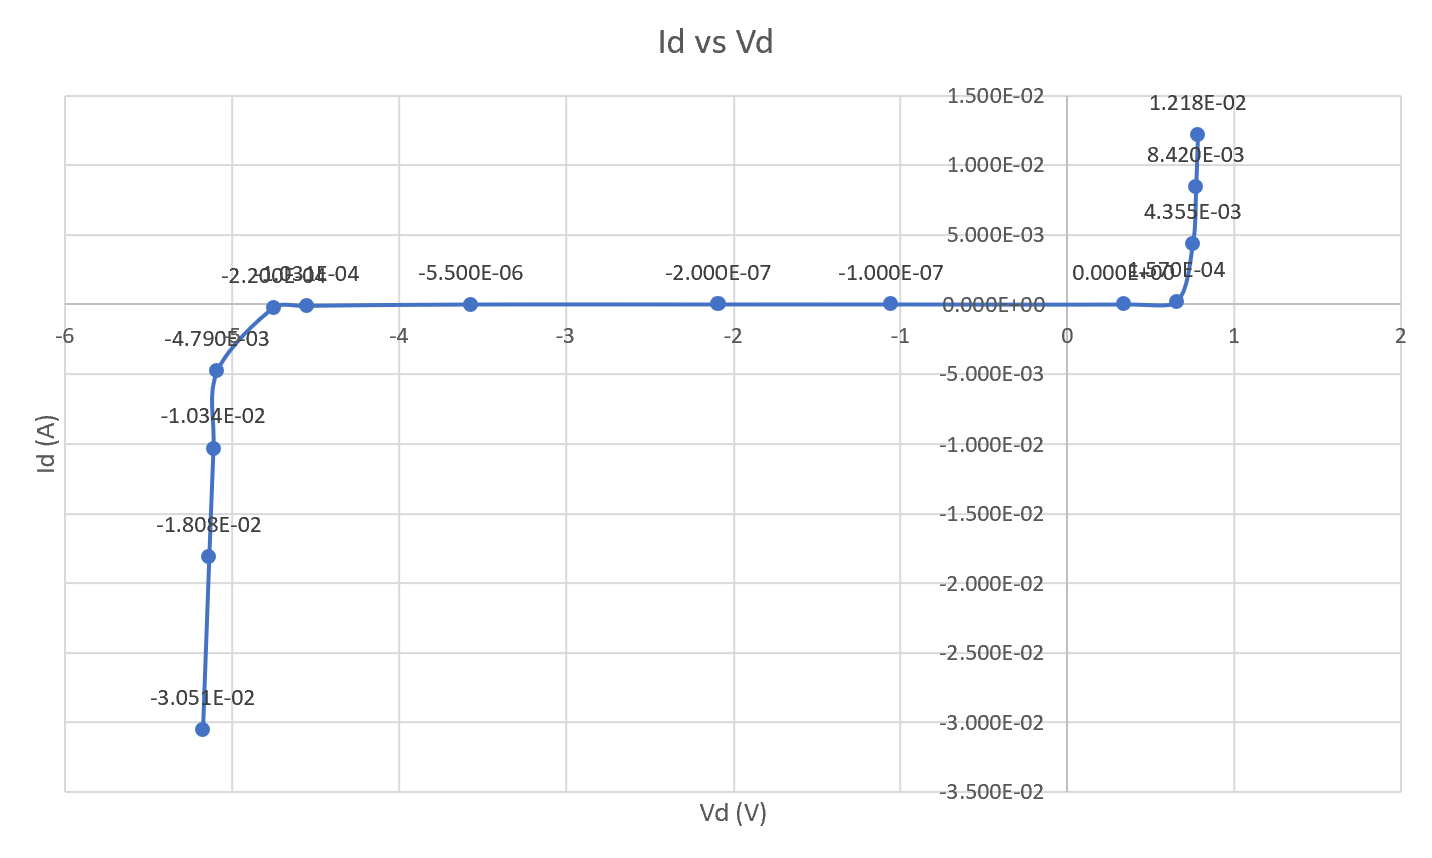
\includegraphics[width=\textwidth]{ECE2200L_Lab4_IV.png}
  \caption{IV chart of 1N4733 Zener Diode}
  \label{fig:IV}
\end{figure}
\begin{figure}[H]
  \centering
  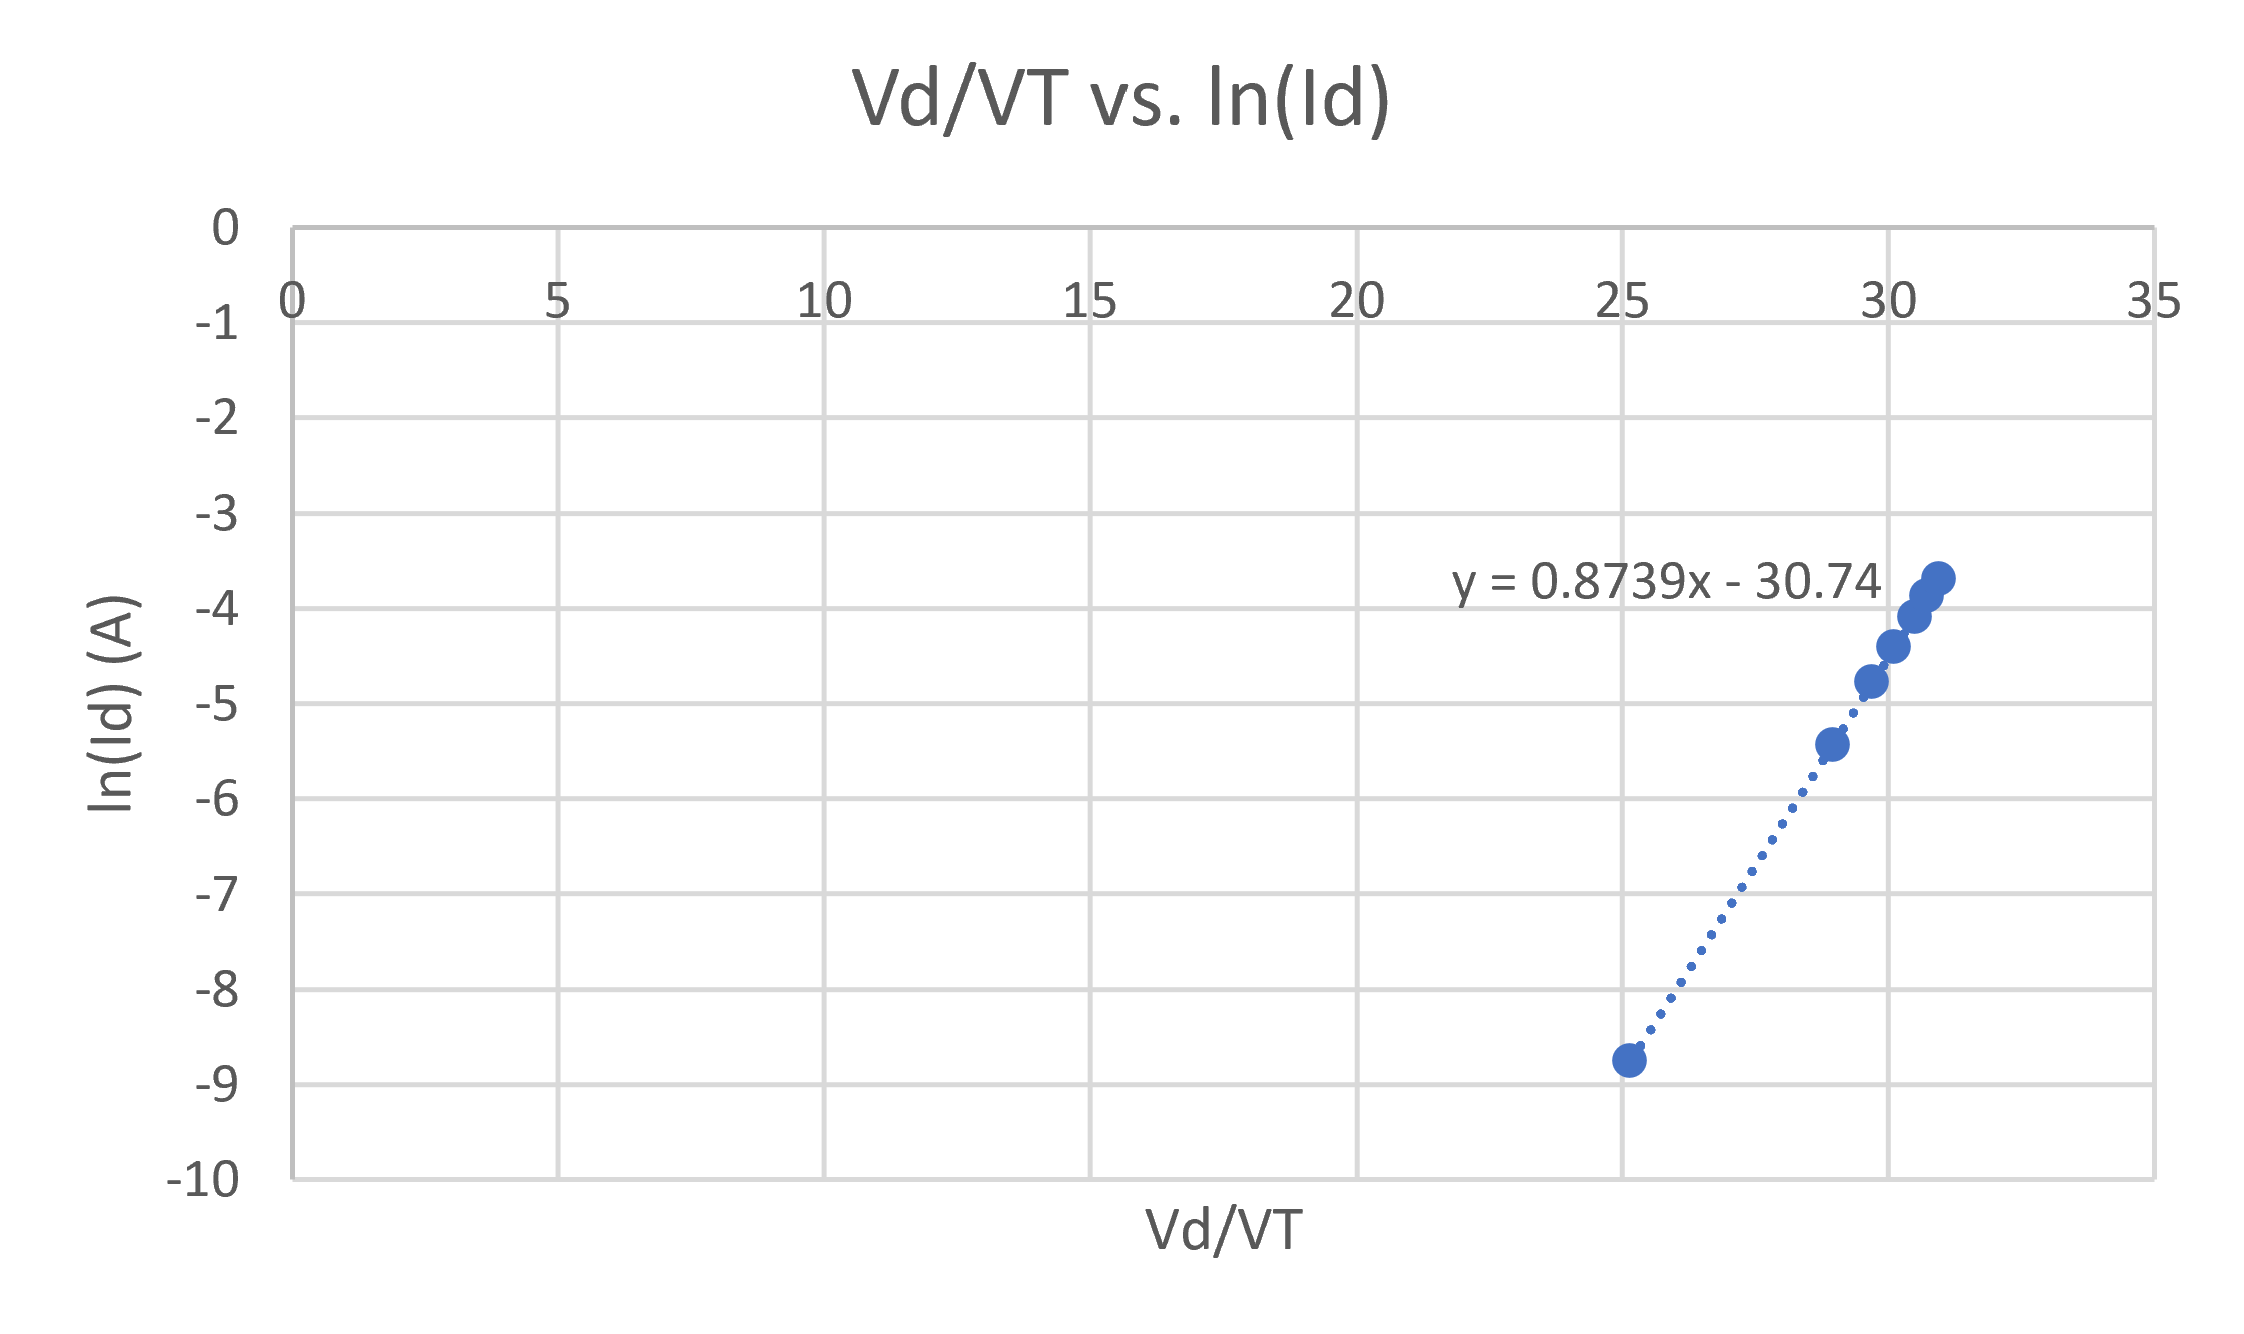
\includegraphics[width=\textwidth]{ECE2200L_Lab4_log.png}
  \caption{$\frac{V_d}{V_T}$ vs $ln(I_d)$ chart of 1N4733 Zener Diode}
  \label{fig:log}
\end{figure}
\begin{figure}[H]
  \centering
  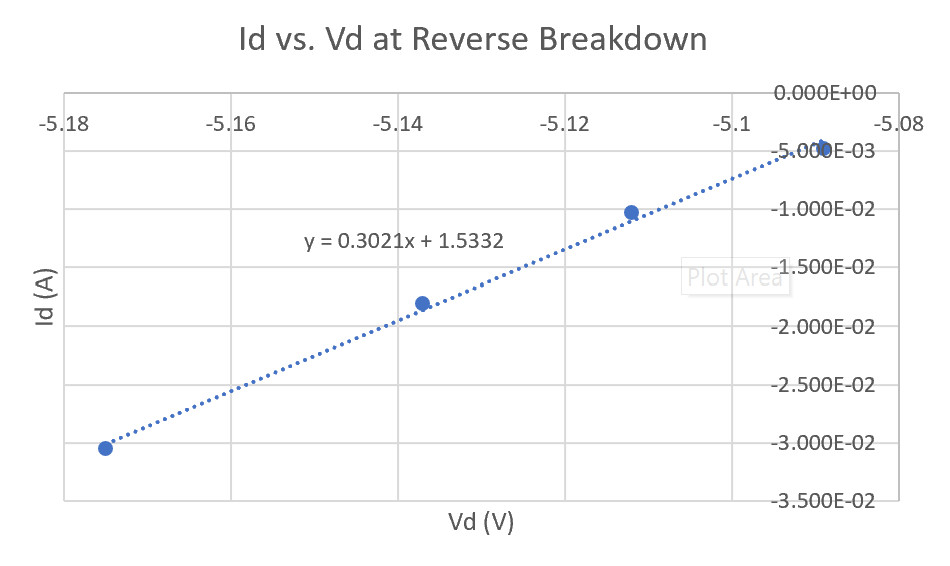
\includegraphics[width=\textwidth]{ECE2200L_Lab4_IV_Breakdown.png}
  \caption{IV chart of 1N4733 Zener Diode at reverse breakdown region}
  \label{fig:breakdown}
\end{figure}
\begin{figure}[H]
  \centering
  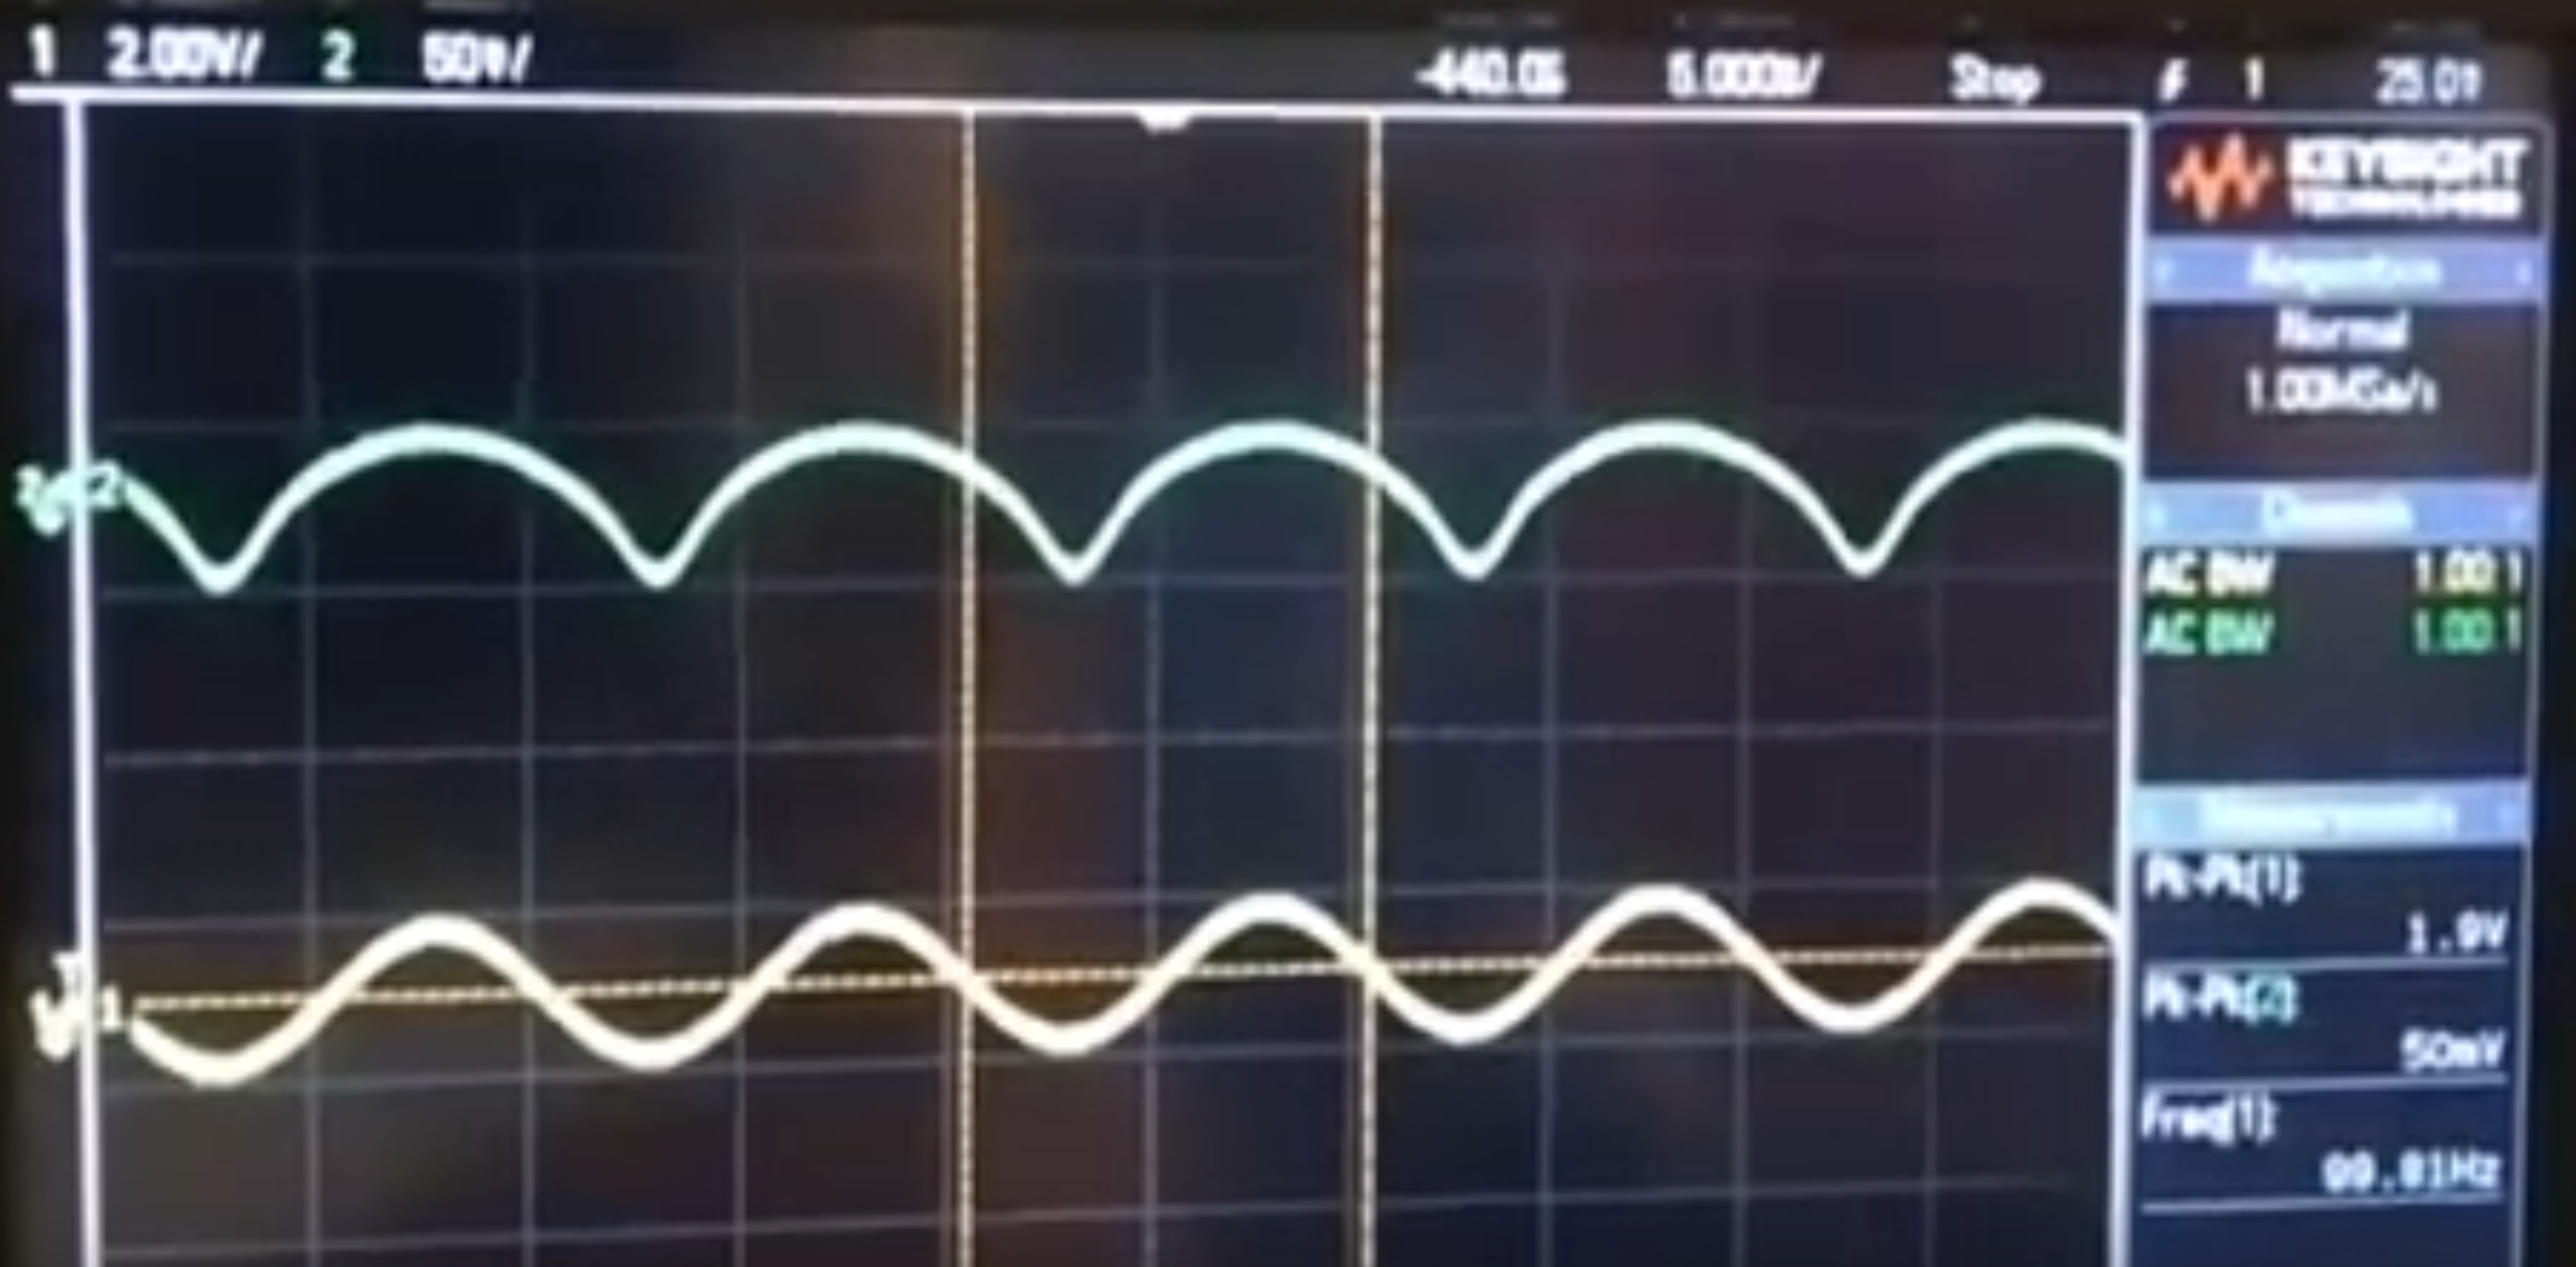
\includegraphics[width=\textwidth]{ECE2200L_Lab4_scope.png}
  \caption{Oscilloscope displaying source and output voltage of part 3 circuit}
  \label{fig:scope}
\end{figure}
The AC component of the source coltage and output voltage measured in part 3 are $V_S = \SI{1.9}{\volt}$ and $V_O = \SI{50}{\milli\volt}$. The Regulator Rejection Ratio is then:
$$RRR=20\log_{10}\left(\frac{V_O}{V_S}\right)=20\log_{10}\left(\frac{0.050}{1.9}\right)=\SI{-31.6}{\deci\bel}$$
\begin{figure}[H]
  \centering
\begin{circuitikz}
  \draw
  (0,0) to[sV_=$V_S$] (0,-2)
  (0,0) to[R=\SI{220}{\ohm}] (2,0)
        to[R=$R_Z\equal\SI{3.31}{\ohm}$]  (2,-2)
  (2,0) -- (6,0)
        to[R=\SI{1}{\kilo\ohm}, v=$V_O$] (6,-2)
        -- (0,-2) node [ground]{}
        ;
\end{circuitikz}
\caption{Small signal model of part 3 circuit}
\label{fig:smallsignal}
\end{figure}

The RRR can also be derived from the small signal analysis using Zener resistance:

$$RRR=20\log_{10}\left(\frac{V_O}{V_S}\right)=20\log_{10}\left(\frac{R_Z||1000}{220+(R_Z||1000)}\right)=20\log_{10}\left(\frac{3.3}{223.3}\right)=\SI{-35.8}{\deci\bel}$$


\section*{Conclusion}
As can be seen above, the ideality factor and Zener resistance can be derived from the IV characteristic chart of the Zener diode. Also, the RRR derived from measured value is higher than the RRR derived from small signal model of the circuit. This could be a result of noise increasing the magnitude of output voltage that in turn increased the output to source voltage ratio.


\end{document}
